% Import the LaTeX style file and load some common packages
\documentclass[final]{siamart1116}
\usepackage{amsfonts}
\usepackage{amsopn}
\usepackage{listings}
\lstset{language=R}
\usepackage{xcolor}

% Declare the title, author, and any other front matter

% Title
\title{Applications of Mathematics in Finance}

% Authors: Full names and addresses
\author{Corbin Apple, Bridget Hyland, Ben Sterling}

% Page headers (visible after the cover page)
\headers{AMS 572 Group Project}{C. Apple, B. Hyland, B. Sterling}

% Start the document
\begin{document}
\maketitle

\section{Introduction}

It has been well established by The United States Environmental Protection Agency and other independent organizations that average temperature is increasing across the country. This study examines monthly temperature data from two stations: Rye Patch Dam, Nevada, and Salt Lake City International Airport, Utah. These stations were chosen because they are roughly at the same latitude ($40.498^{\circ}$N and $40.790^{\circ}$N), longitude ($118.316^{\circ}$W and $111.980^{\circ}$W), and elevation ($1260.3$m and $1287.8$m, for Rye Patch Dam and Salt Lake City respectively). Our data is from the National Centers for Environmental Information (NCEI, a subsidiary of the National Oceanic and Atmospheric Administration) Global Summary of the Month (GSOM) dataset (Lawrimore, Jay H.; Ray, Ron; Applequist, Scott; Korzeniewski, Bryant; Menne, Matthew J. (2016): Global Summary of the Month (GSOM), Version 1. [indicate subset used]. NOAA National Centers for Environmental Information. https://doi.org/10.7289/V5QV3JJ5. [access date]), which contains monthly data about major meteorological parameters at many locations across the country. We chose Salt Lake City and Rye Patch Dam because of their similar geographical characteristics. Data for Rye Patch Dam begins in 1935, but data for Salt Lake City only reaches back to 1948, so we used only years from 1948 to 2020 in our analysis. The dataset includes many parameters, but of particular interest to us were average temperature, average precipitation, number of days with thunderstorms, and total minutes of sunshine.

The goal of our first hypothesis was to examine whether the effects of climate change statistically differ between these two locations; if they do, we may be able to infer that the climate change is predominantly man-made. We accomplished this by calculating the monthly temperature anomaly at each location and comparing the mean temperature anomalies of the two locations. 

The goal of our second hypothesis was to determine predictors of temperature. We used a multiple linear regression with temperature as the response variable and precipitation, days with thunderstorms, and minutes of sunshine as the dependent variables.

\section{First Hypothesis}

Climate change is a well-documented phenomenon: on average, the global temperature is increasing. We wanted to test the hypothesis that the temperature is increasing at a faster rate in Salt Lake City than in Rye Patch Dam. Practically, we tested the hypothesis that the mean temperature anomaly of Salt Lake City is greater than the mean temperature anomaly in Rye Patch Dam.

Temperature anomaly is used to compare change in temperature over time. A mean temperature is calculated over a long period of time, and this long-term mean is subtracted from more recent observations. For example, it is known that the gloval average temperature was $13.9^{\circ}$C between 1901 and 2000. If the global average temperature in 2015 was $14.5^{\circ}$C, then the temperature anomaly for that year would be $14.5 - 13.9 = 0.6^{\circ}$C. When analyzing temperature data over many years, it is advisable to use a temperature anomaly rather than absolute temperature because it eliminates seasonal variation within the year, allowing for a more significant result. This is an accepted and widely used method in climate analysis. \textcolor{red}{[CITE SOMETHING HERE]}

The GSOM records the monthly average temperature at each location, so we determined temperature anomaly monthly. We calculated a January anomaly by averaging the January temperatures of each year from 1948 to 1974. Then, we subtracted this long-term mean from each January temperature from 1975 to 2020. We did the same for the other eleven months and for both locations, yielding different anomalies for each. In our data files, this is column CG, labeled TAVG ADJ. We used this anomaly in our comparison in place of the absolute temperature. It served to reduce the variance of each sample to produce a meaningful result.

Because of the large number of observations in each sample, we invoked the central limit theorem to approximate the distribution as normal. The Shapiro-Wilk test for normality gives a p-value of \textcolor{red}{[P]} for the Salt Lake City sample and \textcolor{red}{[P]} for the Rye Patch Dam sample, which verifies that the normal approximation is appropriate. The normal plots of the temperature anomalies for each station is shown below. The linear nature of the plots further supports our approximation.

Formally, our hypotheses are $$ H_{0}: \mu_{SLC} = \mu_{RPD} \;\; vs. \;\; H_{a}: \mu_{SLC} > \mu_{RPD}.$$ Because the two stations have similar geographical characteristics (i.e. latitude, longitude, and elevation), we determined that this is an observational matched pairs analysis and used the paired t-test at $\alpha = 0.05$ accordingly. As such, it was not necessary to determine equality of variance between the two samples. We determined the test statistic to be $t = \textcolor{red}{[T]}$. This is \textcolor{red}{[GREATER THAN / LESS THAN]} the critical value $t_{n-1,\alpha/2} = \textcolor{red}{[T]}$. Also, the p-value is \textcolor{red}{[P]}, which is \textcolor{red}{[GREATER THAN / LESS THAN]} the confidence level $\alpha = 0.5$. Based on these results, we reject $H_{0}$ and conclude that the mean temperature anomaly at Salt Lake City is significantly greater than the mean temperature anomaly at Rye Patch Dam. In other words, since 1975, the temperature has increased more at Salt Lake City than at Rye Patch Dam. The reason for this is not known, but previous research suggests that Salt Lake City emits a relatively large amount of greenhouse gases per capita, which hastens the effects of climate change there. \textcolor{red}{[CITE SOMETHING HERE]}

We then randomly selected 10\% of the data from each station to remove from the dataset and treat as missing. Although our dataset contains ample missing values on its own, we removed more values in order to evalued the effects of missing data. Our analysis ignored months in which temperature data for Salt Lake City \textit{or} Rye Patch Dam was missing. This resulted in a loss of \textcolor{red}{[N]} data points, leaving us with a new sample size of \textcolor{red}{[N]} for each station. Performing the Shapiro-Wilk test again, the distribution of the observations \textcolor{red}{[WAS STILL NORMAL / WAS NO LONGER NORMAL / WAS STILL NORMAL AT RYE PATCH DAM BUT NOT AT SALT LAKE CITY / WAS STILL NORMAL AT SALT LAKE CITY BUT NOT AT RYE PATCH DAM]}. The new test statistic was \textcolor{red}{[T]}, which is \textcolor{red}{[GREATER THAN / LESS THAN]} the critical value  $t_{n-1,\alpha/2} = \textcolor{red}{[T]}$. The p-value was \textcolor{red}{[P]}, which is \textcolor{red}{[GREATER THAN / LESS THAN]} the confidence level $\alpha = 0.5$. Therefore, we \textcolor{red}{[REJECT H0 / CANNOT REJECT H0]} and \textcolor{red}{[CONCLUDE / DO NOT HAVE SUFFICIENT EVIDENCE TO CONCLUDE]} that the mean temperature anomaly at Salt Lake City is greater than the mean temperature anomaly at Rye Patch Dam. The addition of more missing values reduced the sample size and resulted in a higher p-value, \textcolor{red}{[BUT DID NOT CHANGE / AND CHANGED]} the outcome of the hypothesis test.

\section{Hypothesis 1}

\begin{figure}
  \centering
  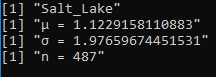
\includegraphics[width=5cm]{../data/img/Salt_Lake_Temp_Diff_Stats.PNG}
  \caption{Statistics for $\Delta T$ in Salt Lake City}
  \label{fig:slc_diff_statistics}
\end{figure}

\begin{figure}
  \centering
  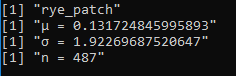
\includegraphics[width=5cm]{../data/img/Rye_Patch_Temp_Diff_Stats.PNG}
  \caption{Statistics for $\Delta T$ in Rye Patch}
  \label{fig:rp_diff_statistics}
\end{figure}

\begin{figure}
  \centering
  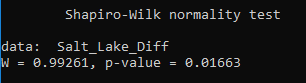
\includegraphics[width=5cm]{../data/img/Salt_Lake_Temp_Diff_Shapiro.PNG}
  \caption{Shapiro-Wilk Normality Test for $\Delta T$ in Rye Patch}
  \label{fig:slc_diff_shapiro}
\end{figure}

\begin{figure}
  \centering
  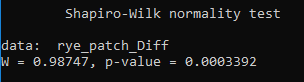
\includegraphics[width=5cm]{../data/img/Rye_Patch_Temp_Diff_Shapiro.PNG}
  \caption{Shapiro-Wilk Normality Test for $\Delta T$ in Rye Patch}
  \label{fig:rp_diff_shapiro}
\end{figure}

\begin{figure}
  \centering
  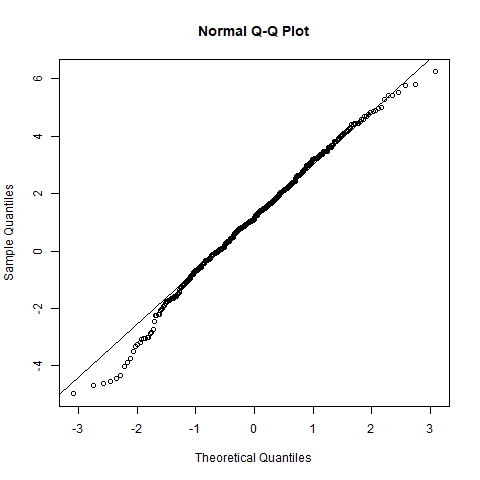
\includegraphics[width=10cm]{../data/img/Salt_Lake_Diff_QQ_Plot.PNG}
  \caption{QQ-Plot for $\Delta T$ in Salt Lake City}
  \label{fig:slc_diff_qqplot}
\end{figure}

\begin{figure}
  \centering
  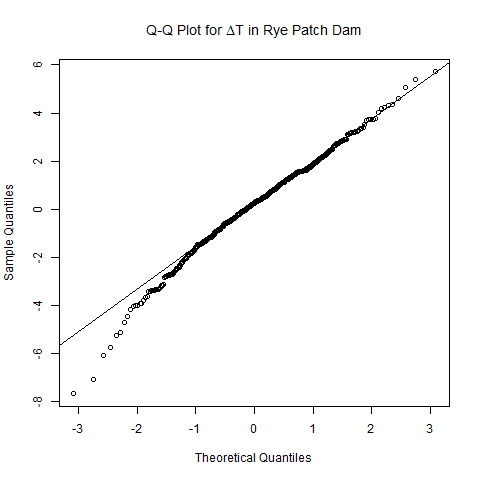
\includegraphics[width=10cm]{../data/img/Rye_Patch_Diff_QQ_Plot.PNG}
  \caption{QQ-Plot for $\Delta T$ in Rye Patch}
  \label{fig:rp_diff_qqplot}
\end{figure}

\begin{figure}
  \centering
  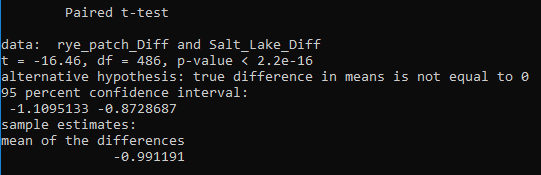
\includegraphics[width=15cm]{../data/img/diff_paired_test.PNG}
  \caption{Paired t-test comparing Salt Lake City $\Delta T$ and Rye Patch $\Delta T$}
  \label{fig:t_test_diffs}
\end{figure}

\section{Hypothesis 2}

\begin{figure}
  \centering
  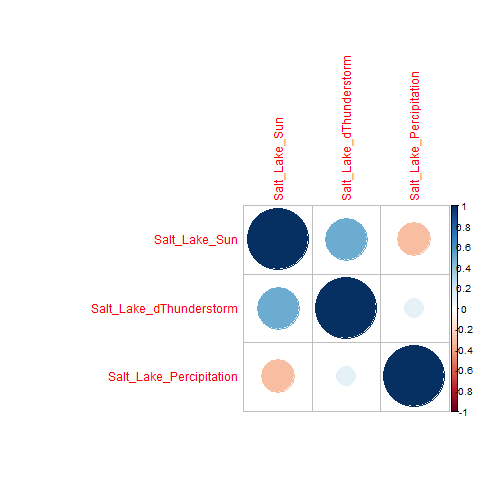
\includegraphics[width=15cm]{../data/img/correlation_plot.PNG}
  \caption{Correlation plot of chosen dependent variables}
  \label{fig:correlation_plot}
\end{figure}

\begin{figure}
  \centering
  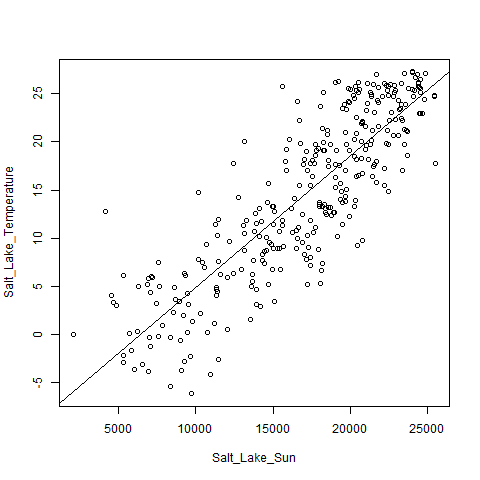
\includegraphics[width=15cm]{../data/img/Temp_vs_sun.PNG}
  \caption{Salt Lake City Temperature versus Sun}
  \label{fig:temp_vs_sun}
\end{figure}

\begin{figure}
  \centering
  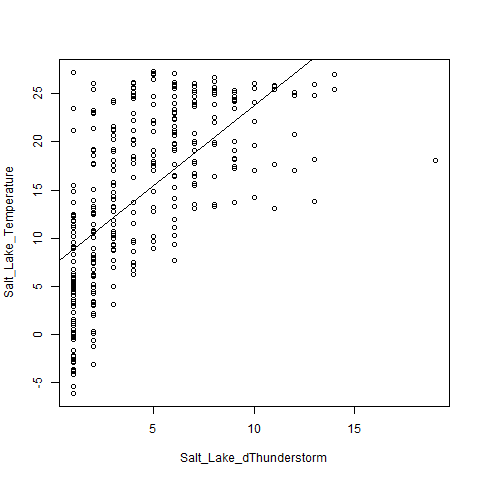
\includegraphics[width=15cm]{../data/img/Temp_vs_dThunderstorm.PNG}
  \caption{Salt Lake City Temperature versus Days of Thunderstorms}
  \label{fig:temp_vs_dthunderstorms}
\end{figure}

\begin{figure}
  \centering
  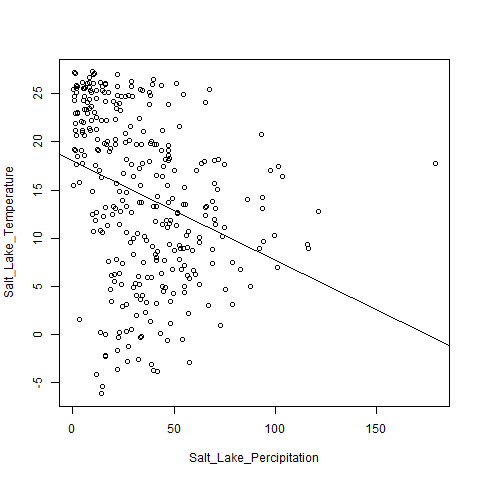
\includegraphics[width=15cm]{../data/img/Temp_vs_Percipitation.PNG}
  \caption{Salt Lake City Temperature versus Percipitation}
  \label{fig:temp_vs_percipitation}
\end{figure}

%\tiny\lstinputlisting{../data/Hypothesis_1.R}

% Put references, in BibTeX format, in the file refs.bib
\bibliographystyle{siamplain}
\bibliography{refs}

\end{document}
